%%\documentclass[pdflatex,sn-basic,Numbered]{sn-jnl}% Basic, numbered refs
%%\documentclass[twocolumn,pdflatex,sn-basic]{sn-jnl}% Basic, two column unnumbered refs
\documentclass[pdflatex,sn-basic]{sn-jnl}% Basic, one column unnumbered refs
%%\documentclass[referee,sn-basic]{sn-jnl}% referee option is meant for double line spacing

%%%% Standard Packages
%%<additional latex packages if required can be included here>

\usepackage{graphicx}%
\usepackage{multirow}%
\usepackage{amsmath,amssymb,amsfonts}%
\usepackage{amsthm}%
\usepackage{mathrsfs}%
\usepackage[title]{appendix}%
\usepackage{xcolor}%
\usepackage{textcomp}%
\usepackage{manyfoot}%
\usepackage{booktabs}%
\usepackage{algorithm}%
\usepackage{algorithmicx}%
\usepackage{algpseudocode}%
\usepackage{listings}%
% \usepackage{lmodern}%
\usepackage{anyfontsize}%
\usepackage{siunitx}%
%%%%

\raggedbottom
\unnumbered% uncomment this for unnumbered level heads

\begin{document}

% Zach's commands

% Units
\DeclareSIUnit{\Molar}{\textsc{m}}
\DeclareSIUnit\uM{\micro\Molar}
\DeclareSIUnit\nM{\nano\Molar}

% Taxonomy
\newcommand\ec{\textit{E.~coli}}
\newcommand\ecfull{\textit{Escherichia coli}}
\newcommand\mtb{\textit{M.~tuberculosis}}
\newcommand\mtbfull{\textit{Mycobacterium tuberculosis}}
\newcommand\msmegfull{\textit{Mycolicibacterium smegmatis}}
\newcommand\pafull{\textit{Pseudomonas aeruginosa}}

% Protein variant and region designations
\newcommand\ftsbTM{FtsB\textsuperscript{TM}}
\newcommand\ftsbLQ{FtsB\textsuperscript{LQ}}
\newcommand\ftsbH{FtsB\textsuperscript{H}}
\newcommand\ftsbdLQ{FtsB\textsuperscript{$\Delta{}$LQ}}
\newcommand\ftsbdH{FtsB\textsuperscript{$\Delta{}$H}}
\newcommand\ftsbdLQdH{FtsB\textsuperscript{$\Delta{}$LQ$\Delta{}$H}}
\newcommand\permN{PerM\textsuperscript{n1}}

% Temp to fill in dummy text
\newcommand\loremipsum{\textcolor{lightgray}{Lorem ipsum dolor sit amet, consectetur adipiscing elit. Nulla volutpat lacus vitae arcu blandit, in maximus arcu bibendum. Aliquam posuere enim et sem egestas gravida. In hac habitasse platea dictumst. Praesent non risus justo. Nullam rhoncus elit in fermentum ultrices. Quisque luctus suscipit lectus in lacinia. Mauris mauris mauris, pretium vitae malesuada id, fringilla aliquet ex. In hac habitasse platea dictumst. Vivamus scelerisque, nulla in euismod placerat, dolor purus commodo tortor, quis congue risus purus nec tellus. Phasellus ultricies lacinia tristique. Duis sollicitudin sapien a nisi sagittis sodales. Suspendisse consequat mauris quis ante consequat tincidunt. Vivamus volutpat in mi vel dictum. Ut ac ligula lectus. Duis ullamcorper ex vitae imperdiet pellentesque. Vestibulum id massa interdum, posuere nibh non, consequat leo.}}

\title[Article Title]{\mtbfull{} FtsB and PerM interact via a C-terminal helix in FtsB to modulate cell division}

\author[1]{\fnm{João Ramalheira} \sur{Ferreira}}
\equalcont{These authors contributed equally to this work.}

\author[1]{\fnm{Ruilan} \sur{Xu}}
\equalcont{These authors contributed equally to this work.}

\author*[1]{\fnm{Zach} \sur{Hensel}}\email{zach.hensel@itqb.unl.pt}

\affil[1]{\orgdiv{ITQB NOVA}, \orgname{Universidade NOVA de Lisboa}, \orgaddress{\street{Av. da República}, \city{Oeiras}, \postcode{2780-157}, \country{Portugal}}}

\abstract{Latent infection by \mtbfull{} impedes effective tuberculosis therapy and eradication. The protein PerM is essential for chronic \mtb{} infections in mice and acts via the divisome protein FtsB to modulate cell division. Using transgenic co-expression in \ecfull{}, we studied the \mtb{} PerM-FtsB interaction in isolation from other \mtb{} proteins, engineering PerM to enhance expression in the \ec{} membrane. We confirmed the reported instability of \mtb{} FtsB and linked FtsB instability to a segment of FtsB predicted to bind cell-division proteins FtsL and FtsQ. Though narrowly conserved, the FtsB-PerM interaction emerges as a potential target as part of therapy targeting persistent infections by disregulating cell division. Using fluorescence microscopy, we found that the stability of both FtsB and PerM hinges on their interaction via a C-terminal helix in FtsB. Molecular dynamics results supported the observation that FtsB stabilized PerM, and suggested that interactions at the PerM-FtsB interface differ from our initial structure prediction in a way that is consistent with PerM sequence conservation. Integrating protein structure prediction, molecular dynamics and single-molecule microscopy, our approach is primed to screen potential inhibitors of the PerM-FtsB interaction and can be straightforwardly adapted to explore other putative interactions.}

\keywords{keyword1, Keyword2, Keyword3, Keyword4}

\maketitle

\section{Introduction}\label{sec1}

\mtbfull{} is a major contributor to preventable deaths by infectious disease and has infected approximately a quarter of the global population \citep{houbenGlobalBurdenLatent2016}. Most infections progress to latent tuberculosis infection (LTBI), characterized by an immunological response to \mtb{} antigens without clinical signs of active TB \citep{whoLatentTuberculosisInfection2018}. Preventing establishment and reactivation of LTBI is a growing priority for TB elimination strategies, although uncertainties continue to limit measurements of the relative burdens of new TB infections and LTBI reactivation \citep{daleQuantifyingRatesLate2021}. Protocols that reduce the duration and adverse effects of treatment can reduce LTBI burden by improving upon completion rates for preventative treatment \citep{assefaEfficacySafetyDifferent2023}. Furthermore, imperfect treatment over long periods can contribute to acquisition of drug resistance \citep{liAcquiredResistanceIsoniazid2021}. Consequently, it is imperative to better understand how \mtb{} infections persist to establish LTBI to inform strategies for novel LTBI treatments with higher efficacy, shorter durations, and reduced risk of drug resistance.

A potential strategy to prevent establishment and reactivation of LTBI is to characterize and target mechanisms through which \mtb{} persists through host-induced stress \citep{dartoisAntituberculosisTreatmentStrategies2022}. The actinomycete protein PerM was one of 21 genes identified in a screen of transposon \mtb{} mutants with attenuated growth at pH~$4.5$ in media containing Tween 80, with most of the identified genes being associated with cell wall synthesis \citep{vandalMembraneProteinPreserves2008}. A subsequent study focused on PerM, finding that Mtb PerM knockout reduced growth during chronic mouse infection and increased $\beta$-lactam antibiotic susceptibility. Localization of fluorescently tagged PerM to dividing septa suggested a connection to cell division \citep{goodsmithDisruptionTuberculosisMembrane2015}. Further work demonstrated that PerM associates with the Mtb divisome, a protein complex orchestrating cell wall remodeling during division, and that PerM depletion can be complemented by overexpression of the divisome component FtsB \citep{wangPersistentMycobacteriumTuberculosis2019}. PerM was also recently identified by transposon sequencing to play an even more significant role in infecting mice in a background with weakened adaptive immune response \citep{meadeGenomewideScreenIdentifies2023}.

Recently, a covalent inhibitor of divisome formation based upon the structure of FtsB-FtsQ was developed and found to be active in vivo against drug-resistant \ec{} \citep{paulussenCovalentProteomimeticInhibitor2022}. The \mtb{} proteome includes homologs of the five core \ec{} divisome proteins FtsQ, FtsL, FtsB, FtsW, and FtsI \citep{wuCharacterizationConservedNovel2018}, suggesting that a similar approach can target protein-protein interactions in the \mtb{} divisome. However, it is unknown whether PerM directly interacts with FtsB  \citep{wangPersistentMycobacteriumTuberculosis2019} and, if it does, whether there is a regulatory mechanism for PerM beyond impacting FtsB stability. PerM lacks known orthologs outside of Actinomycetota \citep{goodsmithDisruptionTuberculosisMembrane2015}, so PerM interactions could potentially be targets of specific therapy. However, no experimental structural data have been published on the PerM-FtsB interaction or on PerM alone to guide experimental design. Expression and purification of Mtb PerM and FtsB for structural study is likely to pose difficulties given that FtsB stability depends upon PerM co-expression in Mtb and \msmegfull{} \citep{wangPersistentMycobacteriumTuberculosis2019}. Furthermore, proteins such as PerM with a high number of transmembrane helices pose challenges for recombinant expression \citep{graveHighthroughputStrategyIdentification2022, korepanovaCloningExpressionMultiple2005}.

Recent insights into the molecular structure and regulatory mechanisms of the gram-negative divisome have been enabled by the confluence of protein structure prediction, cryogenic electron microscopy (Cryo-EM), and molecular dynamics (MD) simulations. The extension from prediction of monomers to protein complexes \citep{baekAccuratePredictionProtein2021, evansProteinComplexPrediction2022} facilitated rapid structure prediction of the core \ec{} divisome \citep{attaibiUpdatedModelDivisome2022, cravenModelInteractionsFtsQLB2022}. Analysis of a Cryo-EM structure of the \pafull{} divisome was largely consistent with predicted protein-protein interfaces, but also revealed a global conformational change absent in structure predictions \citep{kashammerCryoEMStructureBacterial2023}. All-atom MD simulations identified this conformational change within 1 $\mu$s, and further predicted interactions between the core divisome and \ec{} FtsN \citep{brittonConformationalChangesEssential2023}. However, limitations of this MD approach, such as uncertainty in structure predictions and limited MD timescales, call for experimental validation. Importantly, in silico predictions for FtsN were corroborated by experimental results in living cells \citep{parkEssentialDomainFtsN2023}.

In this work, we employed a combination of structure prediction, MD, and fluorescence microscopy to probe the predicted interaction between \mtb{} PerM and FtsB proteins. In our approach, \mtb{} PerM and FtsB were expressed in \ec{} in order to directly attribute observations to changes in the \mtb{} proteins. First, we investigated conservation and dynamics at the predicted PerM-FtsB interface, identifying roles for conserved residues that are absent in structure predictions. Second, we showed that FtsB instability (when expressed in \ec{}) depends on a region predicted to bind FtsL and FtsQ, and that PerM expression in \ec{} can be enhanced by strategically modifying its N-terminal signal sequence. This enabled the quantification of the PerM-FtsB interaction via fluorescence correlation and single-molecule tracking. We found PerM expression in the \ec{} membrane to depend on the FtsB sequence predicted to mediate PerM-FtsB interaction. Lastly, we investigated MD simulations of \mtb{} divisome complexes suggestive of PerM regulatory complexity beyond FtsB stabilization.

\section{Results}

\loremipsum{}

Paragraph introducing approach and perhaps pointing to methods for sequences used and plasmids generated and so on.

\subsection{Structure prediction and molecular dynamics of PerM-FtsB interaction}

\loremipsum{}

Qualitative description and definition of TM (DeepTMHMM prediction), LQ (region with predicted interactions with FtsQ and FtsL and homologous to experimentally observed interactions), H (hydrophobic, helical region predicted to interact with PerM).
Check out Fig.~\ref{fig1_1}A for description of regions of FtsB.

Note similar predictions are observed for diverse homologous sequences (supplementary fig with $pLDDT$ shown for different complexes)

Summary aMD protocol and describe FtsBLQ collapse and loss of predicted conformation with \ftsbTM{} while maintaining and appearing to strengthen interaction with \ftsbH{}.
All simulations using \mtb{} sequences (ref supp table)
Fig.~\ref{fig1_1}A shows aMD results for PerM\textsuperscript{61--204} and FtsB\textsuperscript{11--390}

\begin{figure*}[h]
\centering
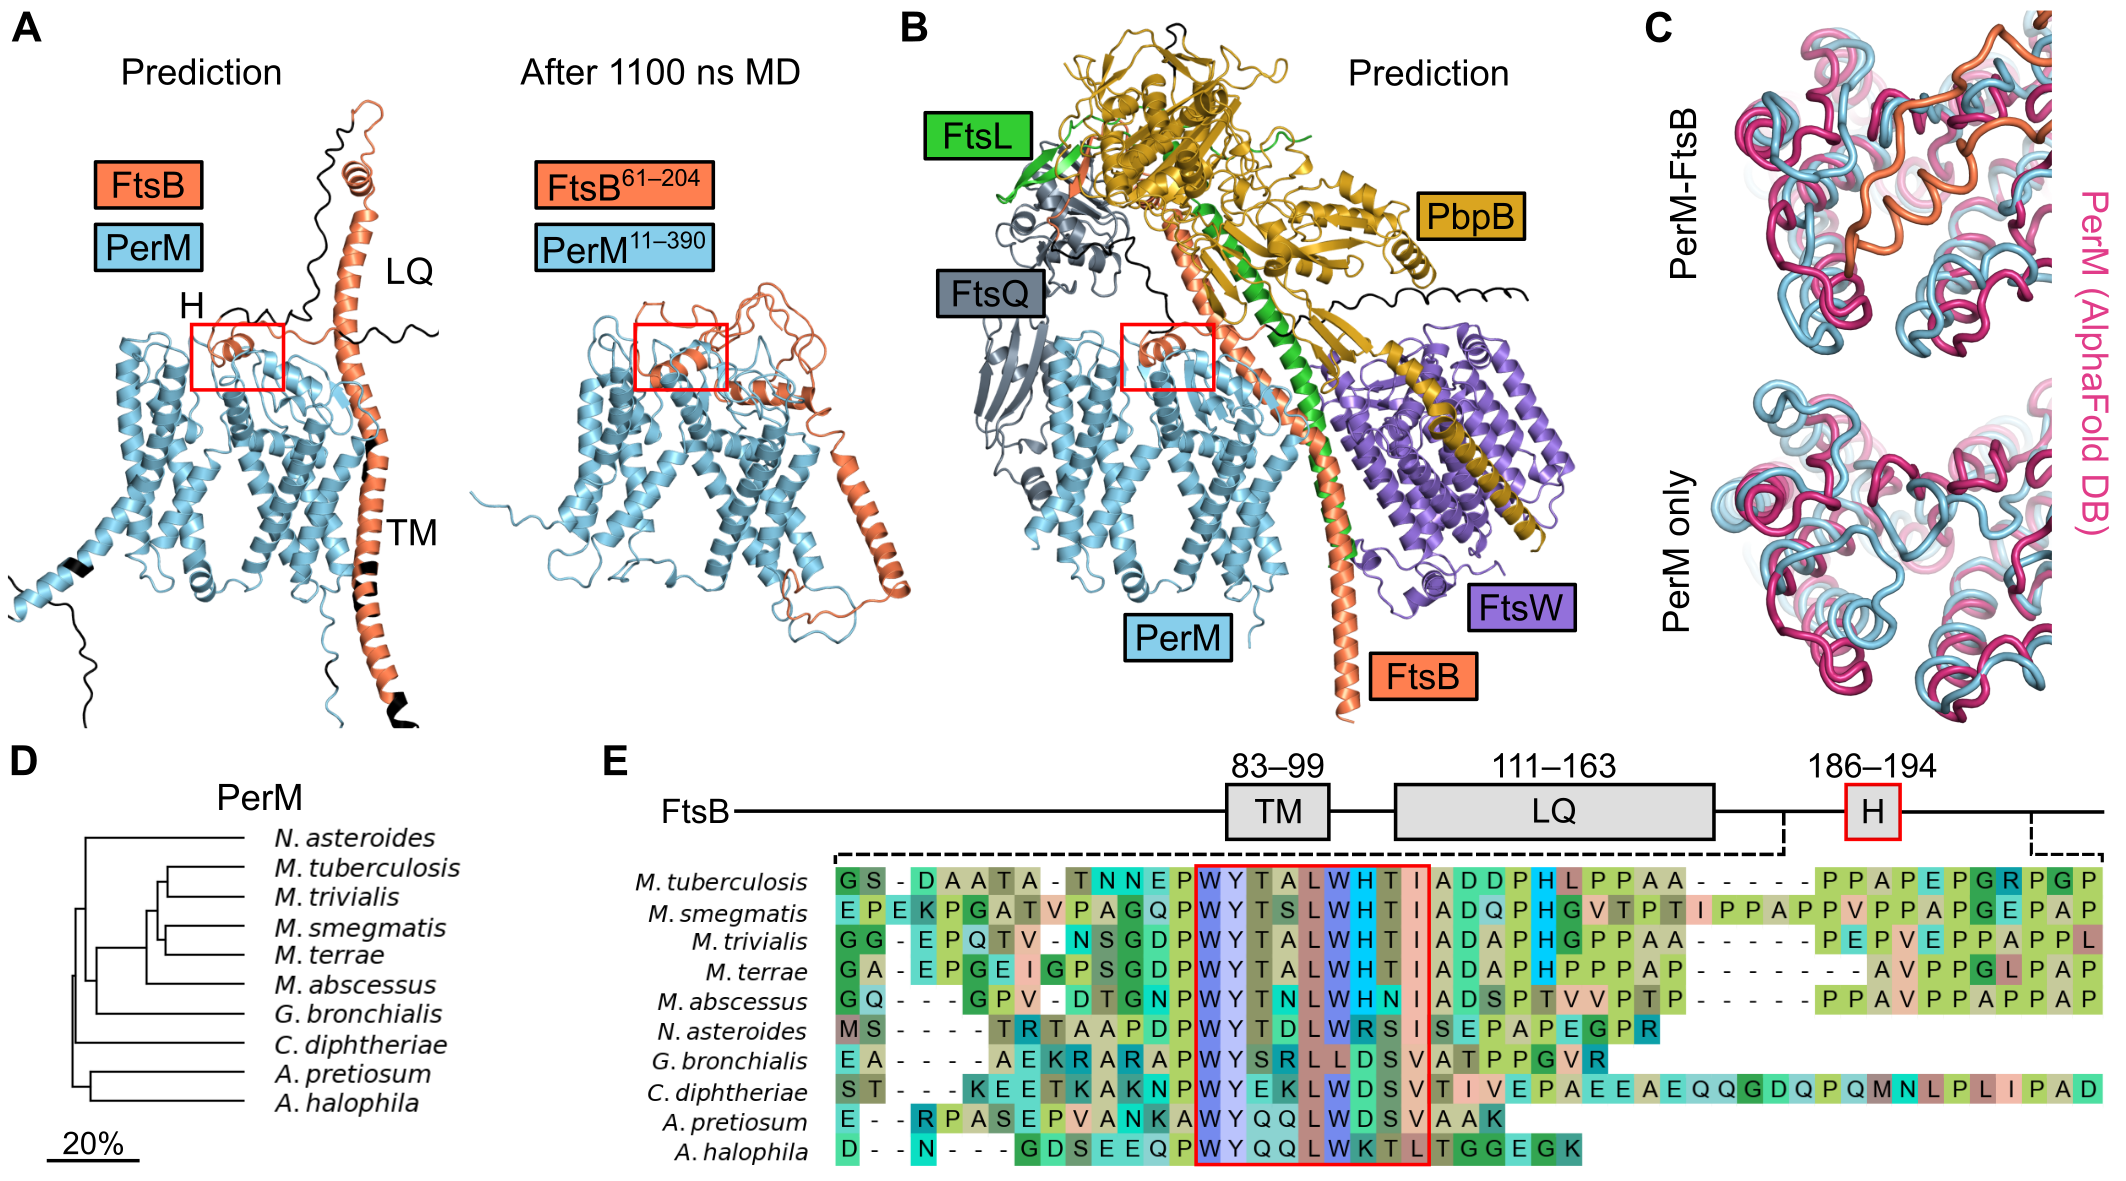
\includegraphics[width=1.0\textwidth]{../figures/fig1_1.png}
\caption{\textbf{A conserved, predicted \mtb{} PerM-FtsB interaction stabilizes PerM in MD.} (\textbf{A})~Left: predicted PerM-FtsB complex in which an $\alpha$~helix, \ftsbH{}, interacts with the periplasmic face of PerM. Transmembrane helix \ftsbTM{} and the region interacting with FtsL and FtsQ, \ftsbLQ{}, are indicated. Residues with $pLDDT < 50$ colored black. Right: final conformer following \qty{1.1}{\ns} MD; PerM-\ftsbH{} interact persists, \ftsbLQ{} collapses, and \ftsbTM{} moves away from PerM. (\textbf{B})~Prediction for the \mtb{} divisome with inclusion of PerM. Terminal regions with $pLDDT < 50$ are omitted except for the FtsB C-terminus. All complexes in \textbf{A} and \textbf{B} are aligned by PerM C$\alpha$ atoms; the red box is placed at the same position relative to PerM for comparison of \ftsbH{} movement. (\textbf{C})~Final MD conformers for PerM-FtsB and FtsB alone are aligned by PerM C$\alpha$ atoms and compared to a PerM prediction  (AlphaFold DB P9WKN3-F1-model{\_}v4). (\textbf{D})~Phylogenetic tree for actinomycete species with predicted PerM-FtsB interactions. Branch length scaled by divergence in amino acid identity in pairwise sequence alignments. (\textbf{E})~Top: Diagram of \mtb{} FtsB defining the \ftsbTM{}, \ftsbLQ{}, and \ftsbH{} regions. Bottom: Multiple sequence alignment of a region near the C-terminus of FtsB for actinomycete species illustrates conservation of residues in \ftsbH{} and diversity in FtsB C-termini.}\label{fig1_1}
\end{figure*}

\loremipsum{}

PerM predicted in context of full divisome using full-length sequences.
Shown in Fig.~\ref{fig1_1}B.

%% Note full length divisome sequences used for this prediction but MD used earlier predictions lacking terminal sequences

Fig.~\ref{fig1_1}C compares final conformers after 1.1~ns aMD for simulations of PerM alone and PerM-FtsB to a PerM structure prediction from the AlphaFold DB (REF AF DB?).
Describe qualitatively differences.
Quantify RMSD.
% RMSD METHODS NOTES HERE; use to write methods later
Raise a question here prompted by observation that PerM-FtsB looks more like AFDB than PerM alone MD... what is FtsB stabilizing?

Reproductible MD results Check out Fig.~\ref{fig1_2}!
Describe binding pocket maturation.
Describe degree of conservation of G228.
Describe hydrogen bonds to residues identified in ~\ref{fig1_1}E as strongly conserved.
Yet these residues are not hydrogen bonded in the predicted dimer structure.
Instead both the W186 binding pocket and hydrogen bonding with conserved FtsB residues emerge during MD simulation. Both were reproducible in replication of the aMD protocol ~\ref{fig1_2}B.

\begin{figure*}[h]
\centering
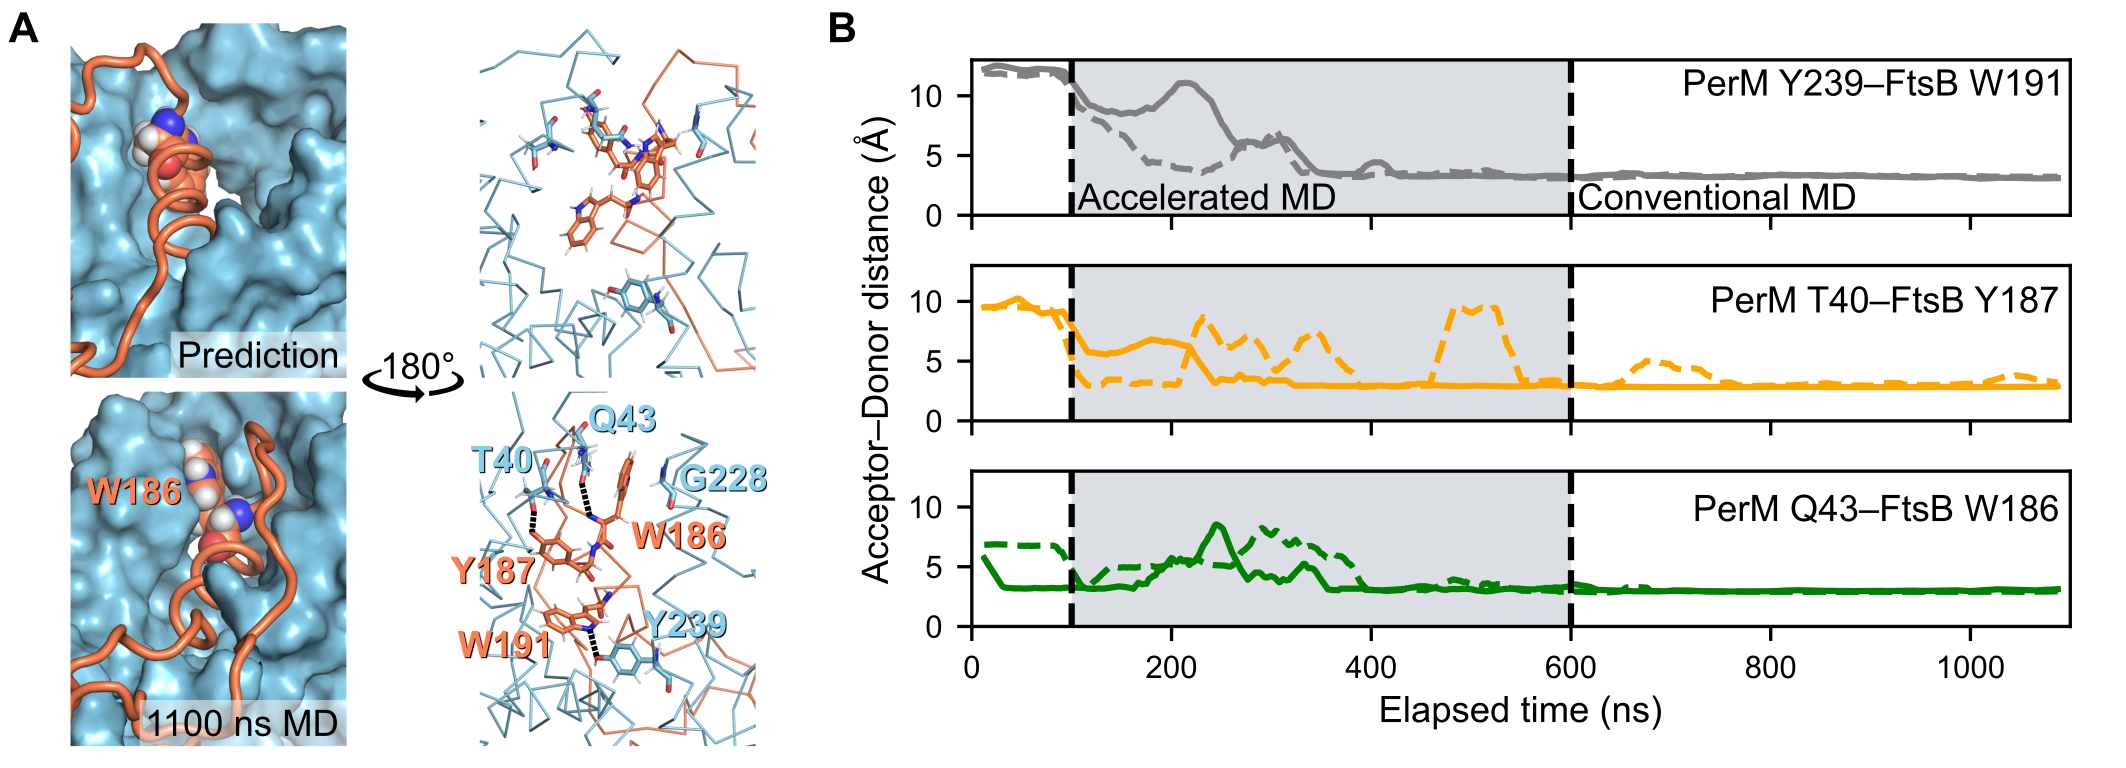
\includegraphics[width=1.0\textwidth]{../figures/fig1_2.png}
\caption{\textbf{Reproducible dynamics at the PerM-FtsB binding interface.} (\textbf{A}) The shape of the FtsB binding pocket for PerM is compared between the predicted interface structure (top) and the final conformer following 1.1~ns MD (bottom). Left: a large predicted periplasmic binding pocket in PerM evolves to tightly bind FtsB W186. Right: Following MD, FtsB W186 interacts with conserved PerM residue G228 and hydrogen bonds are formed between PerM and conserved FtsB residues. (\textbf{B}) Maturation of PerM-FtsB interactions were reproducible in MD. Solid and dashed lines show acceptor-donor distance (25-ns moving average; two MD replicates) for hydrogen bonds at the PerM-FtsB interface that are absent in the predicted structure.}\label{fig1_2}
\end{figure*}

\subsection{FtsB and PerM expression}

Introduce short names for proteins and describe strains and exprimental approach.
Reference supplemental table with strain details.

Check out Fig. \ref{fig2}!

\loremipsum{}

\subsubsection{PerM N-terminal modification}

\loremipsum{}

\begin{figure}[h]
\centering
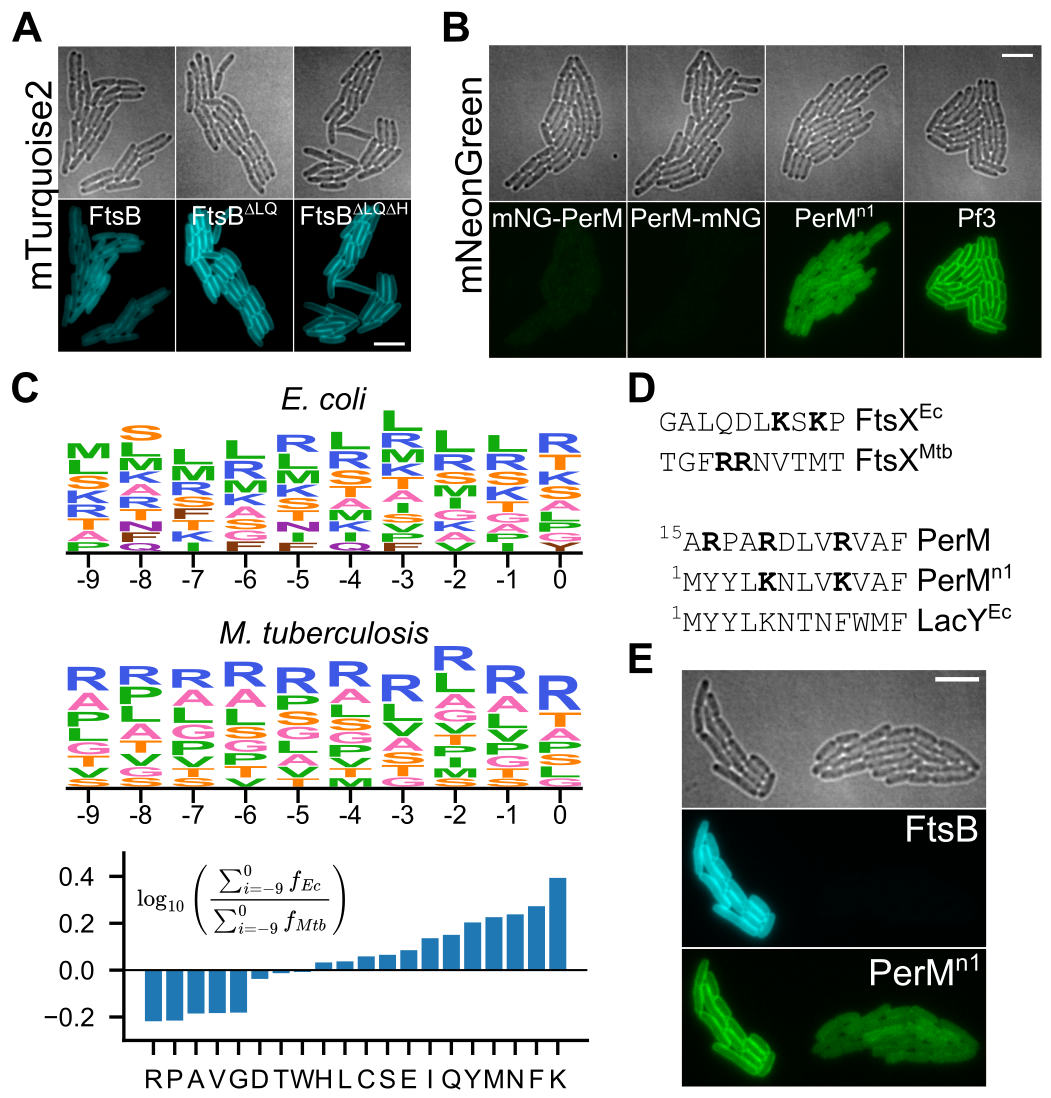
\includegraphics[width=0.5\textwidth]{../figures/fig2.png}
\caption{\textbf{Expression of \mtb{} FtsB and PerM in \ec{}.} (\textbf{A}) Expression and membrane localization of FtsB and variants with deletions of \ftsbLQ{} or with deletion of both \ftsbLQ{} and \ftsbH{}. Identical minimum and maximum intensities for mTurquoise2 images. (\textbf{B}) Expression and membrane localization for mNG-PerM, PerM-mNG, \permN{}-mNG, and Pf3-mNG. Identical minimum and maximum intensities for mNeonGreen images. (\textbf{C}) Top: residue frequency for positions preceding the first predicted transmembrane helix, inclusive of residues found at frequencies above \qty{5}{\percent}. Letter height is proportional to residue frequency with more frequent residues on top. Bottom: relative frequencies in \ec{} and \mtb{}. (\textbf{D}) Top: residues preceding the first transmembrane helix in paralogs of FtsX, highlighting lysine and arginine residues. Bottom: comparison of PerM to \permN{} and \ec{} LacY. (\textbf{E}) Two adjacent microcolonies from a strain with co-expression of mTq2-FtsB and \permN{}-mNG. The microcolony on the right has coincidentally lost the plasmid encoding mTq2-FtsB, and exhibits reduced membrane localization of \permN{}-mNG. Scale bars \qty{5}{\um}.}\label{fig2}
\end{figure}

\subsection{PerM stabilization in \ec{} membrane by FtsB depends on \ftsbH{}}

In order to confirm that FtsB increases membrane-localized PerM expression and, if so, to investigate the role of \ftsbH{} in this phenomenon, we co-expressed mNeonGreen- and mTurquoise2-labeled constructs and analyzed fluorescence in \ec{} microcolonies (Fig.~\ref{fig3}). In these experiments, expression of \permN{}-mNG was induced with \qty{100}{\uM} IPTG. Membrane-localization controls mNeonGreen (cytoplasmic) and Pf3-mNG (membrane) were induced with \qty{60}{\uM} and \qty{240}{\uM} IPTG, respectively, to match typical \permN{}-mNG expression levels. Expression of mTurquoise2-labeled FtsB constructs was induced with \qty{10}{\nM} ATc in all conditions except for one condition with no induction (indicated with down arrows in Fig.~\ref{fig3}). Brightfield images of \ec{} cells were segmented and protein concentration was estimated to be proportional to total integrated fluorescence after subtracting background and normalizing by cell size.

\begin{figure*}[h]
\centering
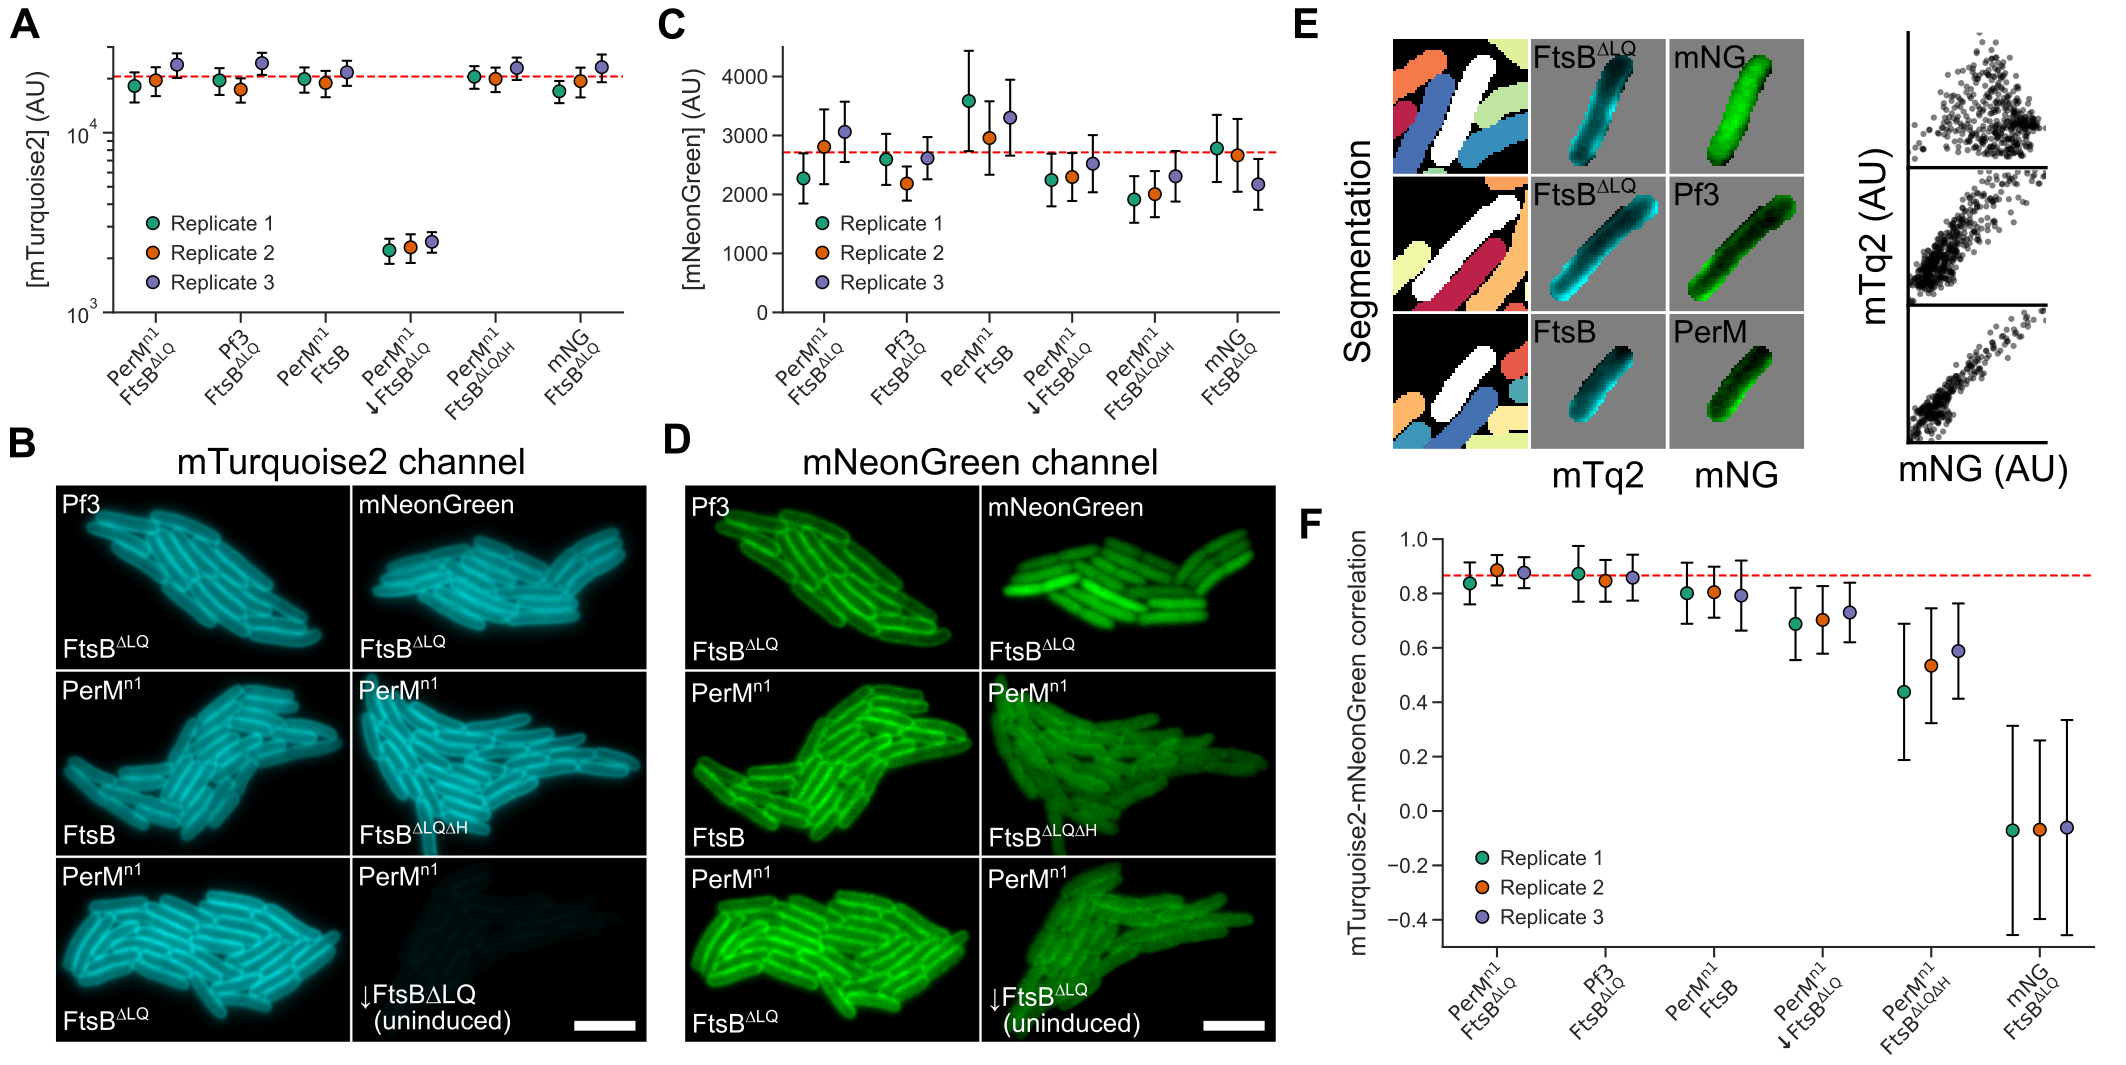
\includegraphics[width=1.0\textwidth]{../figures/fig3.png}
\caption{\textbf{FtsB stabilizes PerM in the \ec{} membrane.} (\textbf{A}) Distribution of single-cell mTurquoise2 concentration (mean $\pm$ standard deviation) for FtsB constructs in different conditions, each with replicates. Dashed red line is the mean value for \permN{} and \ftsbdLQ{} expression with \qty{100}{uM} IPTG. Uninduced \ftsbdLQ{} is indicated with a down arrow. A logarithmic scale is used to allow comparison of high- and low-expression conditions. (\textbf{B}) Example data from microcolonies for each condition. The uninduced \ftsbdLQ{} condition has very low fluorescence in example data because identical minimum and maximum intensities were used. Scale bar \qty{5}{\um}. (\textbf{C,D}) Distribution of single-cell mNeonGreen concentrations and example data for Pf3-mNG, mNeonGreen alone, or \permN{}-mNG in different conditions; prepared identically to \textbf{A} and \textbf{B}. (\textbf{E}) Left: example data analysis showing cell segmentation and isolated, single-cell intensities. Right: Scatter plots of single-pixel intensities for each cell show clear correlation for Pf3-mNG and PerM-mNG, but not for mNeonGreen alone. (\textbf{F}) Distribution of single-cell Spearman correlation coefficients (mean $\pm$ standard deviation) for three replicates.}\label{fig3}
\end{figure*}

Relative to the reference condition (\permN{} and \ftsbdLQ{}, \qty{10}{\nM} ATc), there was an \qty{89}{\percent} ($p=\num{3.3e-12}$) decrease in mTq2-\ftsbdLQ{} expression in the absence of induction, with no significant differences observed for other conditions. The absence of any significant impact on wild-type FtsB expression ($p=0.97$) compared to when FtsB was expressed in the absence of PerM (compare Fig.~\ref{fig3}B to Fig.~\ref{fig2}A) suggests that \permN{} stabilizes FtsB when expressed in \ec{}, as was observed in \mtb{} \citep{wangPersistentMycobacteriumTuberculosis2019}. There was also no obvious difference in localization of any FtsB variant in any condition tested.

In contrast, there was a significant reduction in \permN{}-mNG expression of \qty{13.3}{\percent} ($p=\num{3.8e-2}$) in the absence of induction of mTq2-\ftsbdLQ{} expression, and a reduction of \qty{23.5}{\percent} ($p=\num{5.5e-4}$) when \ftsbdLQ{} was replaced with \ftsbdLQdH{}. There was no significant change when \ftsbdLQ{} was replaced with wild-type FtsB ($p=0.29$). This suggested that FtsB increases PerM stability in \ec{}, and that this depends on the presence of \ftsbH{}. However, inspection of Fig.~\ref{fig3}C suggests that our sample size is overpowered ($N=\num{10930}$ cells in total from 3 replicates; $607 \pm 44$ cells per condition per replicate) given variation between replicates in mNeonGreen expression levels. 

In preliminary experiments, we observed a large decrease in spatial correlation between mTurquoise2 and mNeonGreen fluorescence when \ftsbdLQ{} was depleted or replaced by \ftsbdLQdH{} (Fig.~\ref{fig3}D). The observation of small reductions in mNG-\permN{} levels despite apparently large impacts of different FtsB constructs on localization suggested that fluorescent mNeonGreen often remained in the cytoplasm following mNG-\permN{} degradation. We hypothesized that quantifying spatial correlation would be a more sensitive measurement less susceptible to variation in protein expression levels. Fig.~\ref{fig3}E shows scatter plots of mNeonGreen and mTurquoise2 intensities for pixels in typical cells with cytoplasmic mNeonGreen, membrane-localized Pf3-mNG, and \permN{}-mNG. We calculated Spearman correlation coefficients from such distributions for segmented cells and Fig.~\ref{fig3}F shows the mean and standard deviation of correlation coefficients for each condition and replicate.

In the reference condition (\permN{}-mNG, mTq2-\ftsbdLQ, \qty{10}{nM} ATc), correlation was high ($\rho = 0.87$, 0.84--0.89 \qty{95}{\percent} confidence interval) and indistinguishable from that when Pf3-mNG was expressed instead ($p = 0.72$). All other conditions had significant reductions in correlation. Wild-type FtsB was marginally less well correlated ($\rho = 0.80$, 0.77--0.83). The apparent reductions in \permN{}-mNG expression levels discussed above were more strongly supported by analysis of spatial correlation, with a drops in correlation in the absence of mTq2-\ftsbdLQ{} induction ($\rho = 0.71$, 0.69--0.73) and a larger drop when mTq2-\ftsbdLQ was replaced with mTq2-\ftsbdLQdH ($\rho = 0.52$, 0.46--0.58). While \ftsbLQ{} was not absolutely essential for membrane localization of \permN{}, this was also observed in the absence of any FtsB expression (Fig.~\ref{fig2}B).

\subsection{Single-molecule FtsB tracking}

Our correlation analysis strongly suggested that FtsB interaction with PerM via \ftsbH{} is key for expression of \permN{} in the membrane. Since we observed this for transgenic expression in \ec{}, it is unlikely that PerM-FtsB interaction is mediated by host proteins. However, transient PerM-FtsB interaction could be sufficient for PerM stability without a large fraction of molecules being bound at any time. If PerM is a significant component in the core \mtb{} divisome as suggested by depletion phenotypes and midcell localization \citep{goodsmithDisruptionTuberculosisMembrane2015, wangPersistentMycobacteriumTuberculosis2019}, we hypothesized that this implied long-lived FtsB-PerM interactions that could be detected by single-molecule tracking of FtsB diffusion. FtsB has a single transmembrane helix and PerM is predicted to have 8 (Fig.~\ref{fig1_1}A), suggesting an expected reduction in the FtsB diffusion coefficient from approximately 0.7 to \qty{0.3}{\square\um\per\s} upon PerM binding \citep{lucenaMicrodomainFormationGeneral2018}.

\loremipsum{}

Check out Fig. \ref{fig4}!

\begin{figure*}[h]
\centering
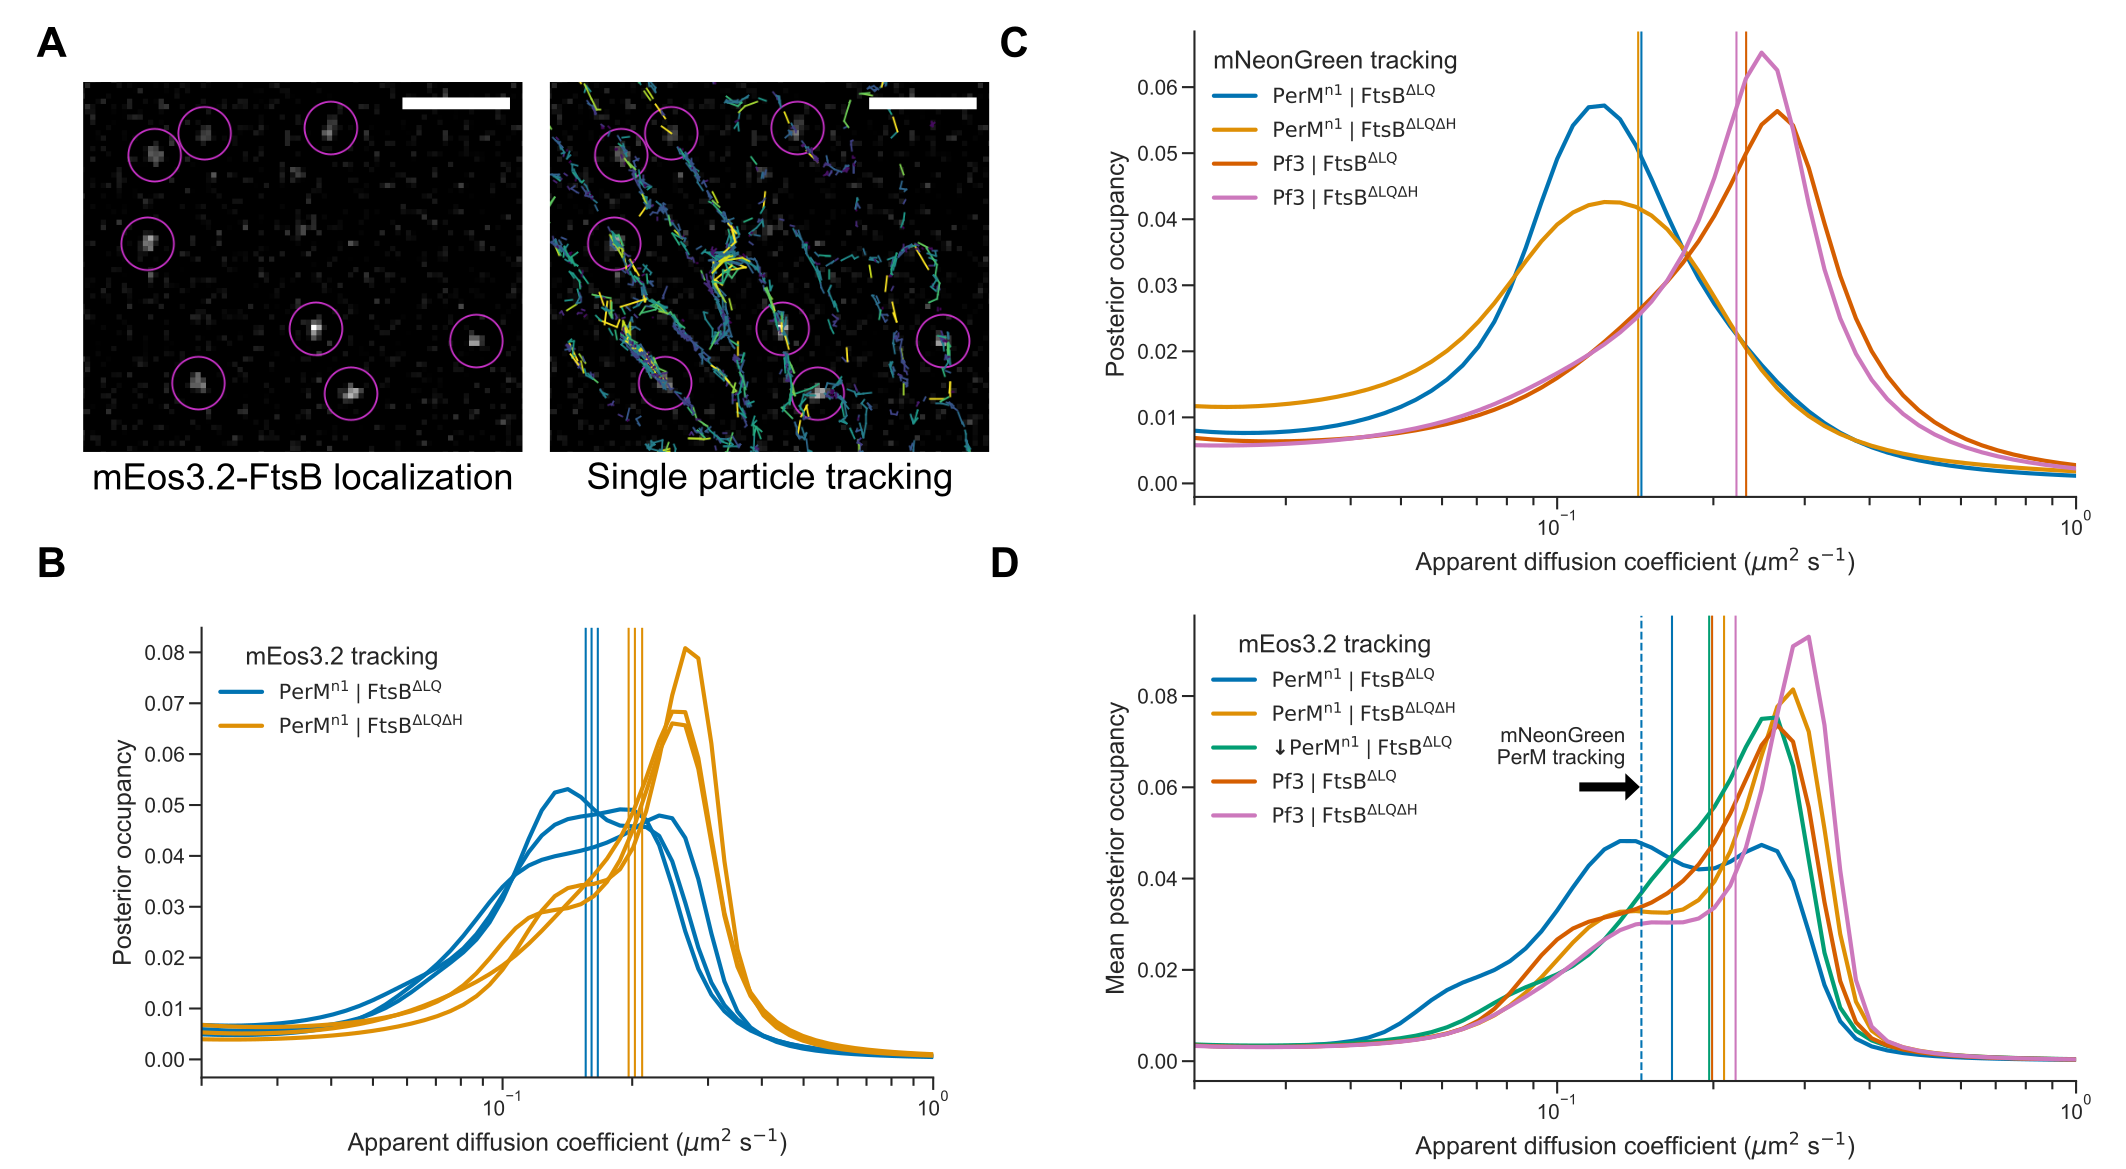
\includegraphics[width=1.0\textwidth]{../figures/fig4.png}
\caption{\textbf{PerM-FtsB binding detected by FtsB single-molecule tracking.} (\textbf{A}) Left: single, 33-ms frame from timelapse fluorescence imaging of mEos3.2-\ftsbdLQ{} diffusion in \ec{}. Right: Single-molecule localization tracks for the entire movie show membrane-localized diffusion. Scale bar $2~\mu$m. (\textbf{B}) Posterior occupancies in a model of regular Brownian motion and localization error were marginalized over localization error to estimate the distribution of apparent 2D diffusion coefficients. Distributions and their means (dashed lines) are shown for three replicates of experiments combining \permN{}-mNG with either mEos3.2-\ftsbdLQ{} or mEos3.2-\ftsbdLQdH{}. (\textbf{C}) Estimated distributions of diffusion coefficients inferred from single-molecule tracking of either \permN{}-mNG or Pf3-mNG with either \ftsbdLQ{} or \ftsbdLQdH{} (single experiment). Dashed line is the mean estimated diffusion coefficient for \permN{}+\ftsbdLQ{}. (\textbf{D}) Mean estimated distribution of diffusion coefficients for either mEos3.2-\ftsbdLQ{} or mEos3.2-\ftsbdLQdH{} co-expressed with either Pf3-mNG or \permN{}-mNG (with or without addition of 100~$\mu$M~IPTG).}\label{fig4}
\end{figure*}

\subsection{Complex MD (fig 5)}

\loremipsum{}

% Figure 5 goes here
% \begin{figure*}[h]
% \centering
% 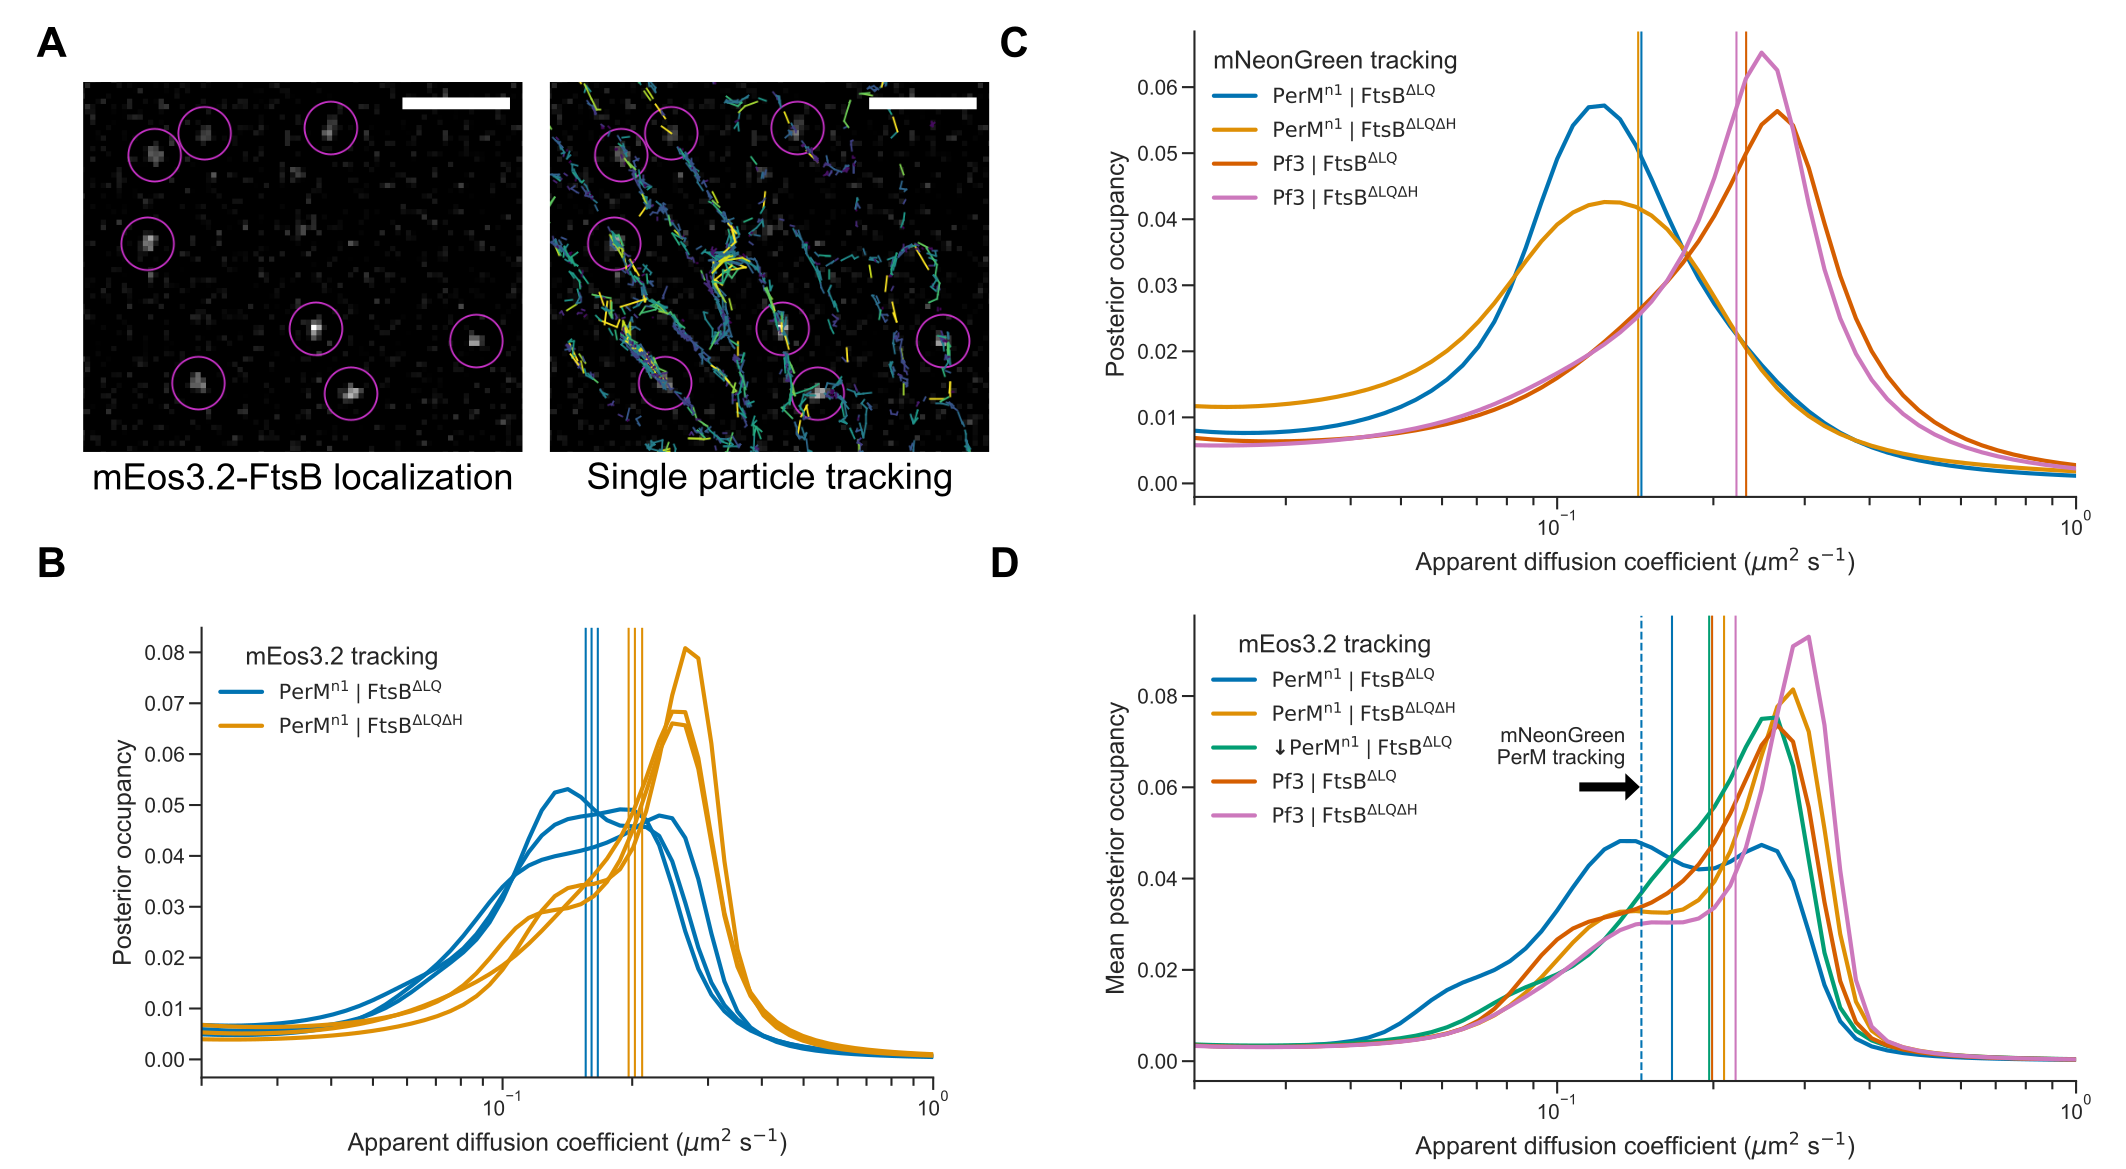
\includegraphics[width=1.0\textwidth]{../figures/fig4.png}
% \caption{PerM-FtsB binding detected by FtsB single-molecule tracking. (\textbf{A}) (\textbf{B}) (\textbf{C}) (\textbf{D})
%     FtsB Tracking caption here.}\label{fig4}
% \end{figure*}

Note region initially predicted and used for MD.

\section{Discussion}

\loremipsum{}

\loremipsum{}

\loremipsum{}

\loremipsum{}

% Recap 

% Limitations

% Overall conclusion

\section{Methods}

\subsection{Structure prediction}

\loremipsum{}

\subsection{Molecular dynamics}

\loremipsum{}

\subsection{Sequence analysis}

\loremipsum{}

\subsection{Strains}

Cloning details.

\loremipsum{} 

\subsection{Microscopy}

Cell growth.
Sample preparation.
Microscope details.

\loremipsum{}

\subsubsection{Microcolony fluorescence imaging}

Sample size.

\loremipsum{} 

\subsubsection{Single-molecule tracking}

\loremipsum{} 

\subsection{Image analysis}

ImageJ/Fiji reference for image preparation.

\loremipsum{}

\subsubsection{Inference of diffusion coefficient distributions}

SASPT details.
Brief discussion of apparent 2D diffusion and challenge of identifying perfect method.
Details needed to define reported values.

\loremipsum{} 

\subsubsection{Microcolony fluorescence correlation}

Background estimation and substraction. Does not effect correlation by definition.
Segmentation of brightfield images with Omnipose.
Image registration. Important.

\loremipsum{} 

\subsection{Statistical analysis}

For mNeonGreen and mTurquoise2 concentration and correlation comparisons, a mixed linear model was fit to data points from single cells with random slopes and intercepts to allow for day-to-day variation. Two-tailed p-values were calculated for comparison to the reference condition (\permN{} and \ftsbdLQ{}, 100~nM~ATc) and adjusted for multiple comparisons using the Holm-Šidák method. Effect sizes are reported for significant results only (adjusted $p<0.05$). Unless stated otherwise, errors in the manuscript are 1 standard error of the mean.

\loremipsum{}

\backmatter

\bmhead{Acknowledgements}

FUNDING. HELP IN LAB (SMC). HELP IN WRITING AND REVIEW. ANY PLASMIDS/REAGENTS?

\bmhead{Resource availability}
Plasmids described in this manuscript will be made available through AddGene shortly.
Analysis code on GitHub.
Data available on request and will be archived to Zenodo following peer review.

\bmhead{Author contributions}

JF: molecular cloning, data acquisition, preliminary data analysis and interpretation. RX: data acquisition, data analysis. ZH: management, structure predictions and simulation, data acquisition, data analysis. All authors wrote and edited the manuscript.

\bibliography{perm-ftsb}% common bib file

\begin{appendices}

\section{Supplementary Figures and Tables}

\begin{figure*}[h]
\centering
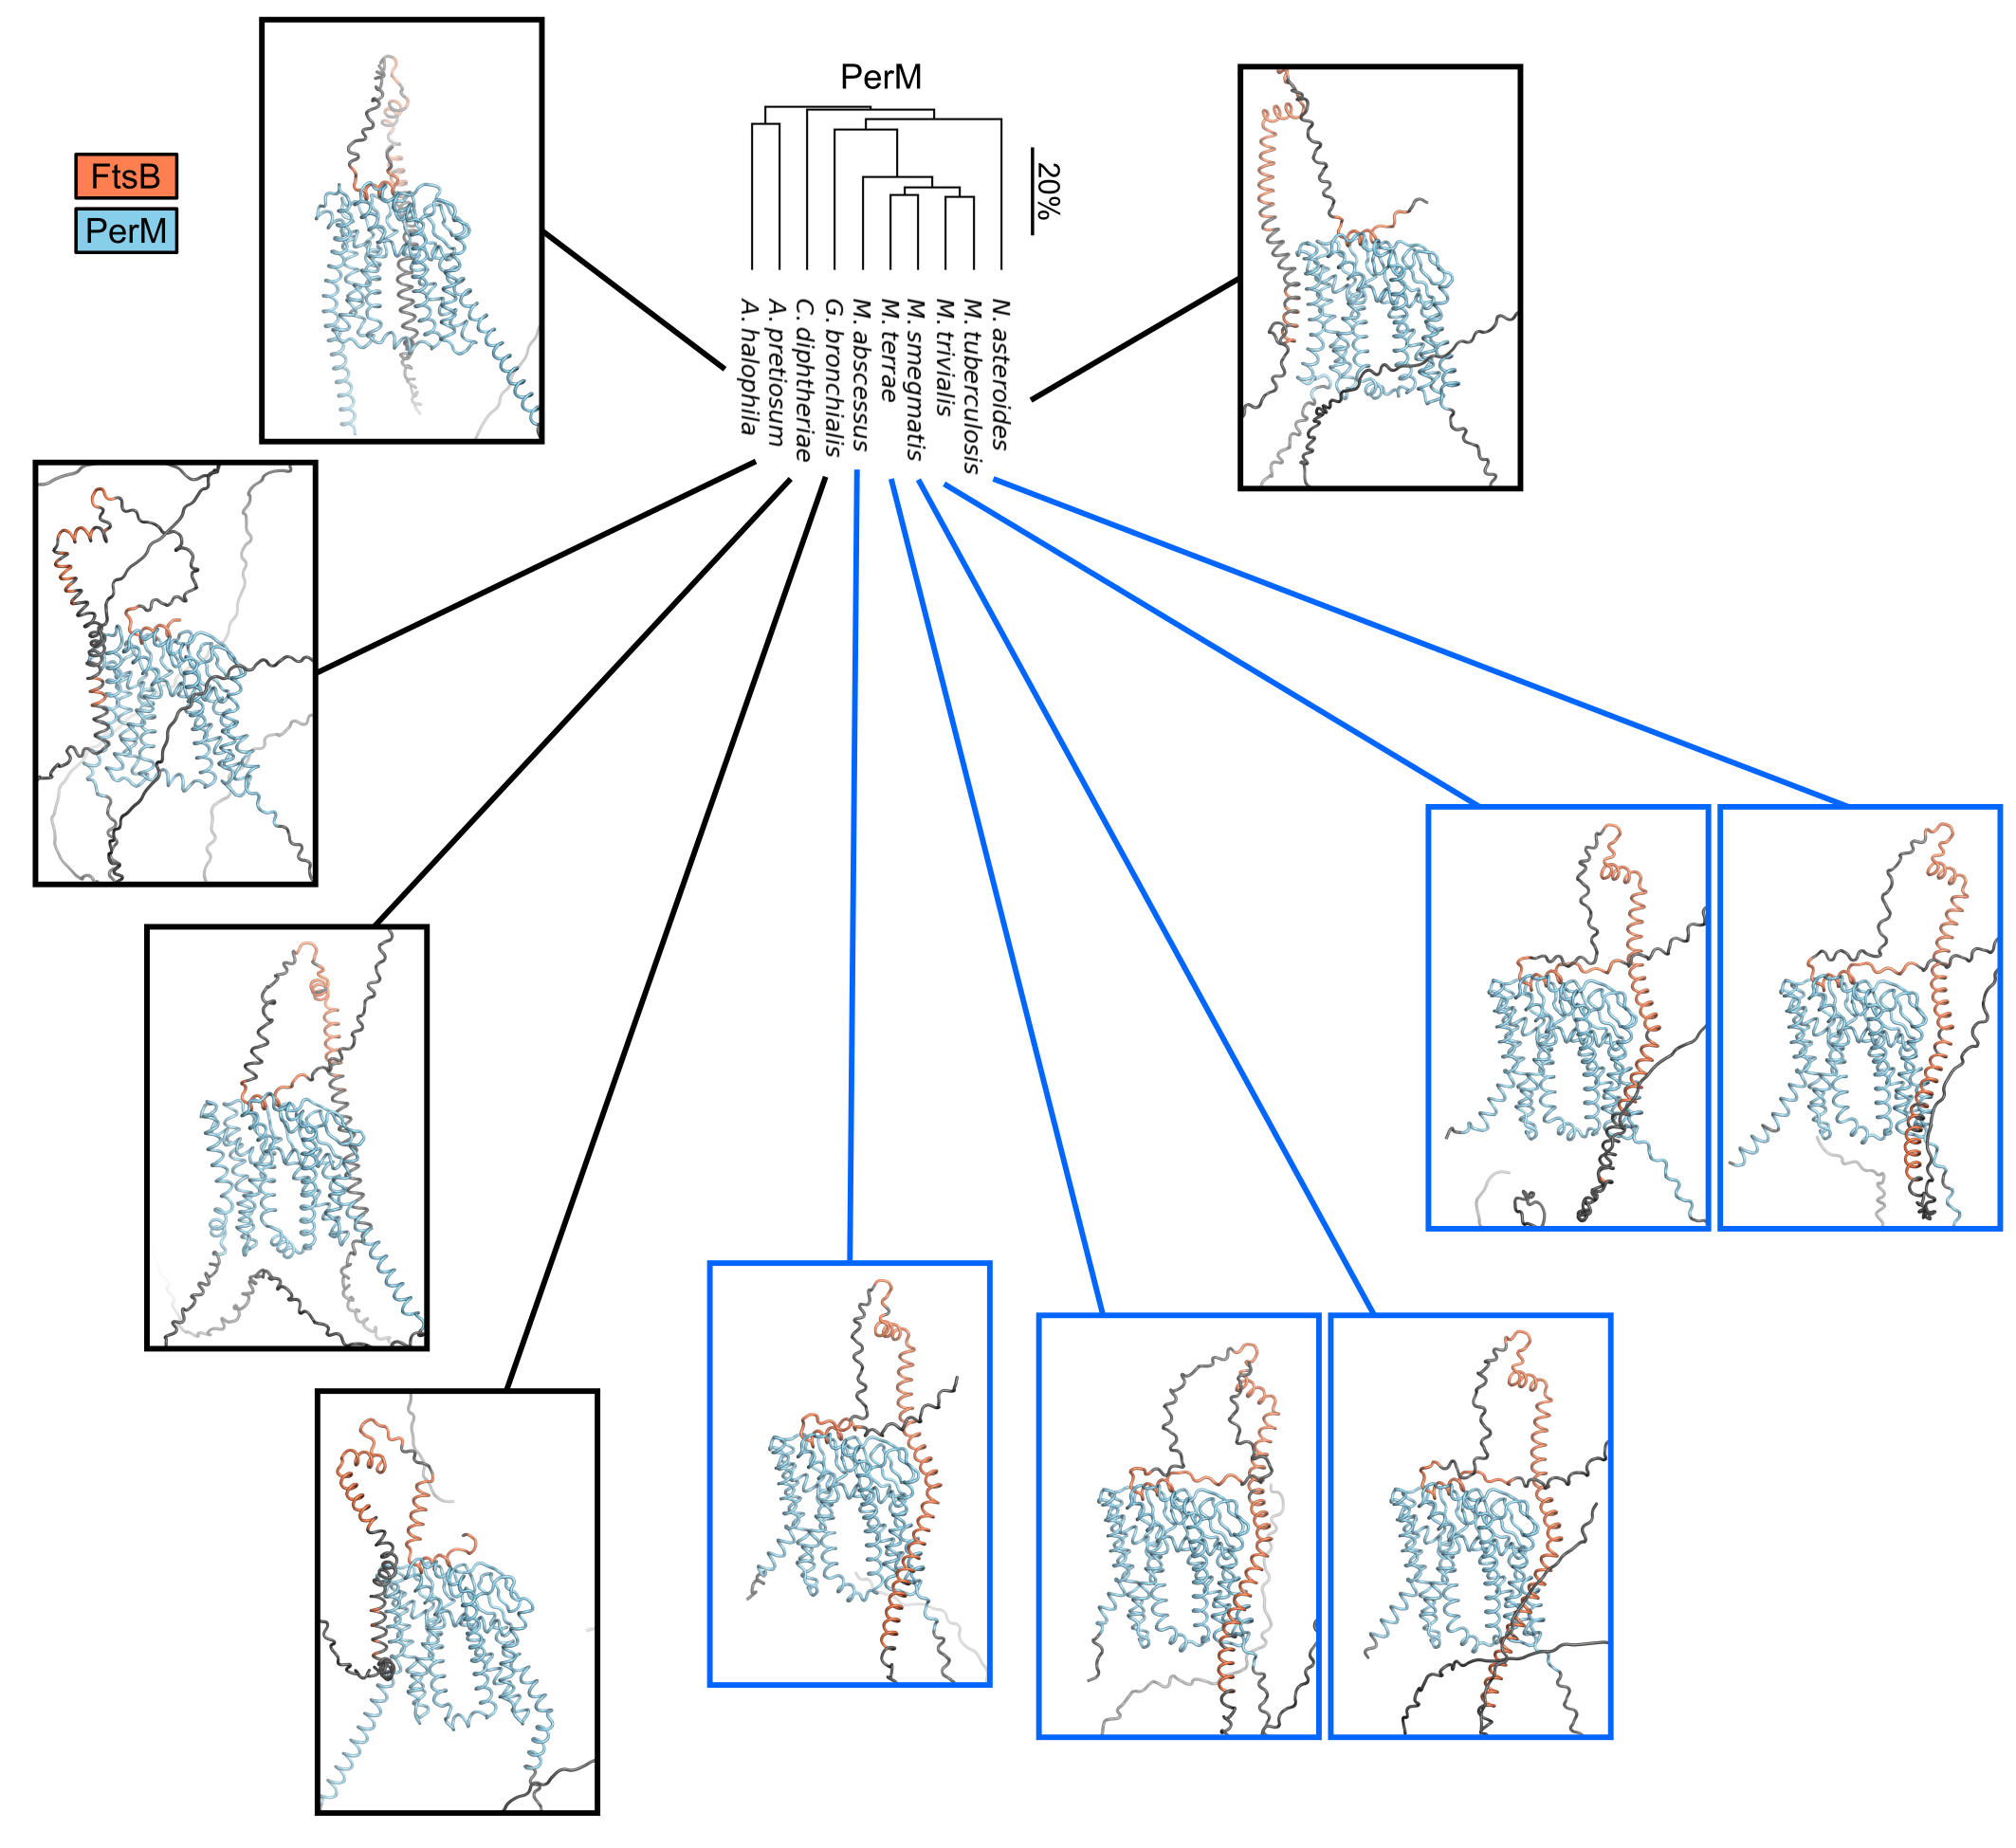
\includegraphics[width=1.0\textwidth]{../figures/figS1.png}
\caption{The PerM phylogenetic tree from Fig.~\ref{fig1_1} is reproduced and compared to PerM-FtsB complexes predicted from full-length sequences for the same species. The predicted orientation of \ftsbTM{} relative to PerM observed for \mtb{} is only observed for more closely related species (blue lines). However, \ftsbH{} interaction with PerM is predicted for all species. Residues with $pLDDT<50$ are colored gray.}\label{figS1}
\end{figure*}

\end{appendices}

\end{document}
